\chapter{Injection and Detection Techniques}

\section{Why Injection Matters in Cheat Development}

In professional game cheating, especially in competitive games like \textit{Counter-Strike 2}, most serious cheats are built as \textbf{DLLs} that are injected into the game's running process.

\begin{tcolorbox}[colback=gray!10, colframe=gray!10, boxrule=0pt, sharp corners, width=\linewidth, left=1mm, right=1mm, top=0.5mm, bottom=0.5mm]
\textbf{What is a DLL?} \\
A DLL (Dynamic Link Library) is like a small add-on that can be loaded into a program to extend what it can do. In the case of cheats, a DLL gives direct access to the game's memory and functions.
\end{tcolorbox}

Injecting a DLL allows the cheat to run \textbf{at the same time} as the game itself. This enables cheats to:

\begin{itemize}
    \item \textbf{Hook game functions} to change behavior (e.g., aiming or vision systems).
    \item \textbf{Modify memory} to adjust gameplay (e.g., speed, ammo, recoil).
    \item \textbf{Read internal data} like player positions or weapon stats.
    \item \textbf{Draw overlays} directly on the screen (e.g., radar, ESP).
    \item \textbf{Automate actions} to perform tasks faster or more accurately.
\end{itemize}

Because of this deep integration, cheat injection is the main focus of anti-cheat systems like \textbf{Valve Anti-Cheat (VAC)}.

\section{Overview of Code Injection Techniques}

\textbf{Code injection} means inserting new code into a running program. In cheat development, this usually means adding a DLL or custom code into the game's memory.

\subsection*{Traditional Methods}

Earlier cheats used simple Windows functions like:

\begin{itemize}
    \item \texttt{LoadLibrary}: Loads a DLL into another process.
    \item \texttt{CreateRemoteThread}: Starts a new thread inside another program.
\end{itemize}

These methods are now easy for anti-cheats to detect because they leave obvious traces.

\subsection*{Manual Mapping}

Today, cheats mostly use a method called \textbf{Manual Mapping}.

\begin{tcolorbox}[colback=gray!10, colframe=gray!10, boxrule=0pt, sharp corners, width=\linewidth, left=1mm, right=1mm, top=0.5mm, bottom=0.5mm]
\textbf{What is Manual Mapping?} \\
Manual Mapping is a way of loading a DLL manually into a program’s memory without using Windows' normal loading functions. This makes it much harder for anti-cheat systems to notice the injection.
\end{tcolorbox}

Manual Mapping avoids showing up in the list of loaded modules and can start execution in stealthy ways, such as by hijacking existing game threads.

\begin{figure}[H]
    \centering
    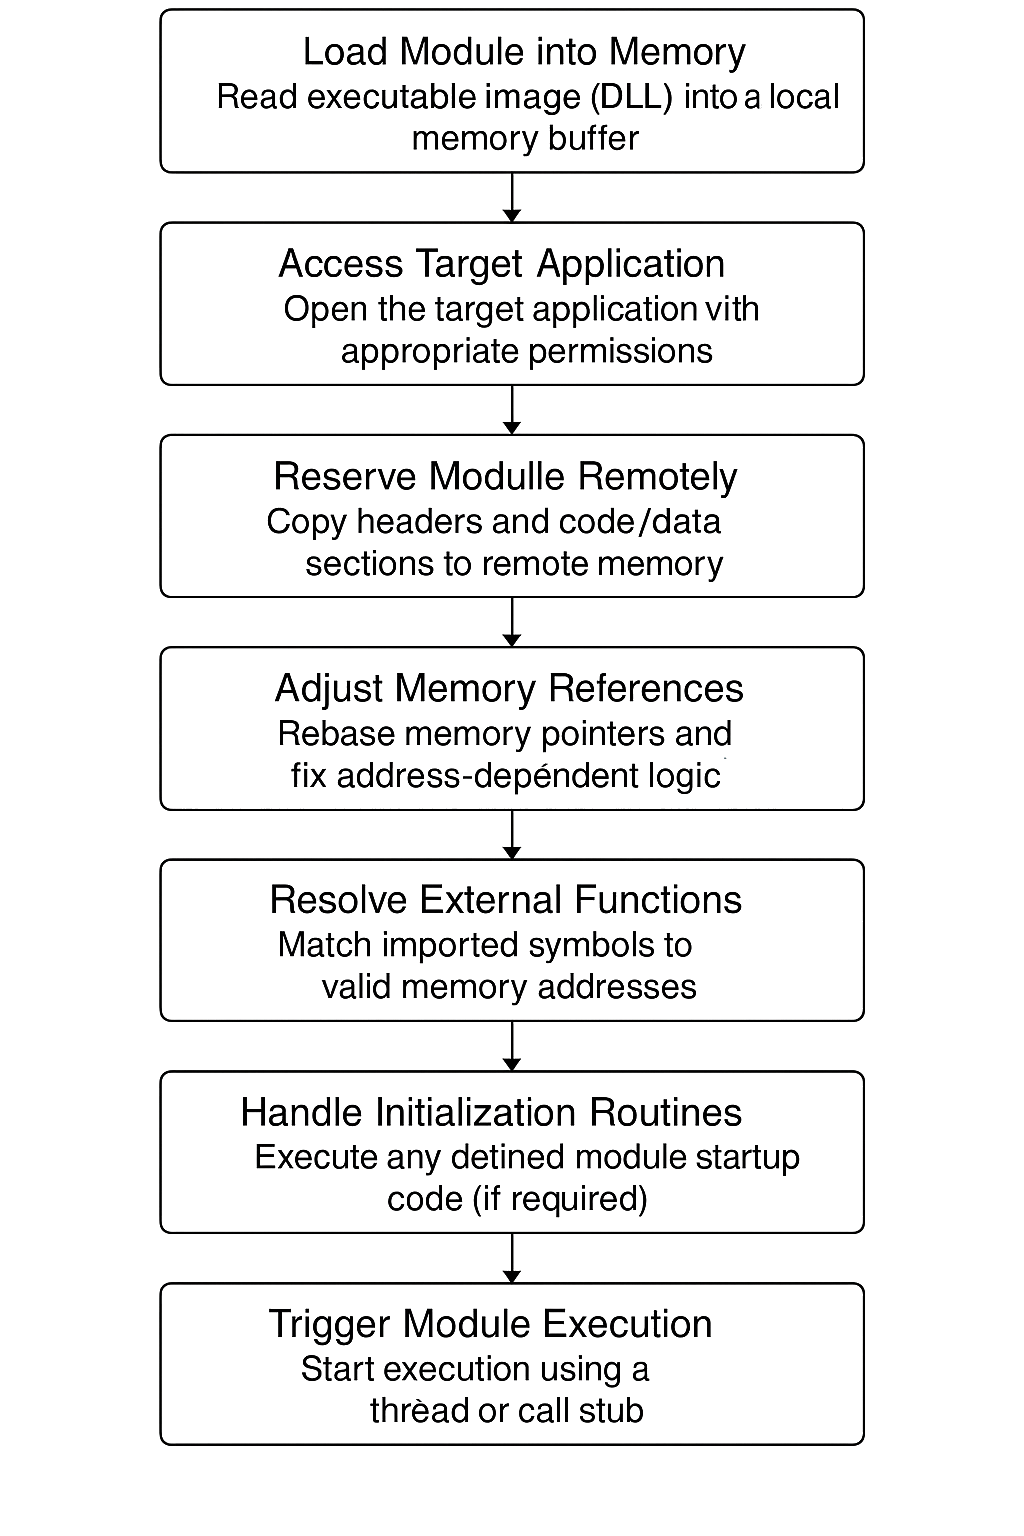
\includegraphics[width=0.60\textwidth]{images/diagram_white_background.png}
    \caption{Simplified flowchart of dynamic module injection using Manual Mapping.}
    \label{fig:manual_mapping_flow}
\end{figure}

We have developed our own injector that follows the structure outlined in Figure~\ref{fig:manual_mapping_flow}.  
The source code for this injector can be found in the \texttt{injector} branch of the project repository.

\section{Detection Techniques in Anti-Cheat Systems}

The detection techniques described in this section are \textbf{not merely theoretical}; they are the result of \textbf{practical reverse engineering} carried out on modules \textit{extracted (dumped)} directly from the game's memory during runtime.  
Through detailed analysis of the internal workings of \textbf{Valve Anti-Cheat (VAC)}, we have gathered \textbf{concrete evidence} supporting the mechanisms and strategies presented below.

Modern anti-cheat systems, such as VAC, deploy a wide range of methods to detect the presence of unauthorized code within game processes.  
These methods are specifically designed to identify \textit{abnormal memory modifications}, \textit{injected modules}, or \textit{manipulation of trusted system structures}.

In the following sections, we outline and explain the principal detection techniques observed during our research.

\subsection*{Thread Local Storage (TLS) Callbacks}

One early opportunity for anti-cheats to detect injected code occurs during program startup.  
When a program or DLL starts running, Windows can automatically execute special functions known as \textbf{TLS callbacks}.

\begin{tcolorbox}[colback=gray!10, colframe=gray!10, boxrule=0pt, sharp corners, width=\linewidth, left=1mm, right=1mm, top=0.5mm, bottom=0.5mm]
\textbf{What is a TLS Callback?} \\
A TLS (Thread Local Storage) callback is a special function that Windows automatically calls when a thread starts, before the main application code runs. Developers can use it for initialization tasks — but it can also be leveraged by anti-cheats for early memory inspections.
\end{tcolorbox}

Anti-cheats leverage this early execution stage to scan memory and inspect the runtime environment, often before the main game code even begins.

\begin{comment}
\begin{figure}[h!]
    \centering
        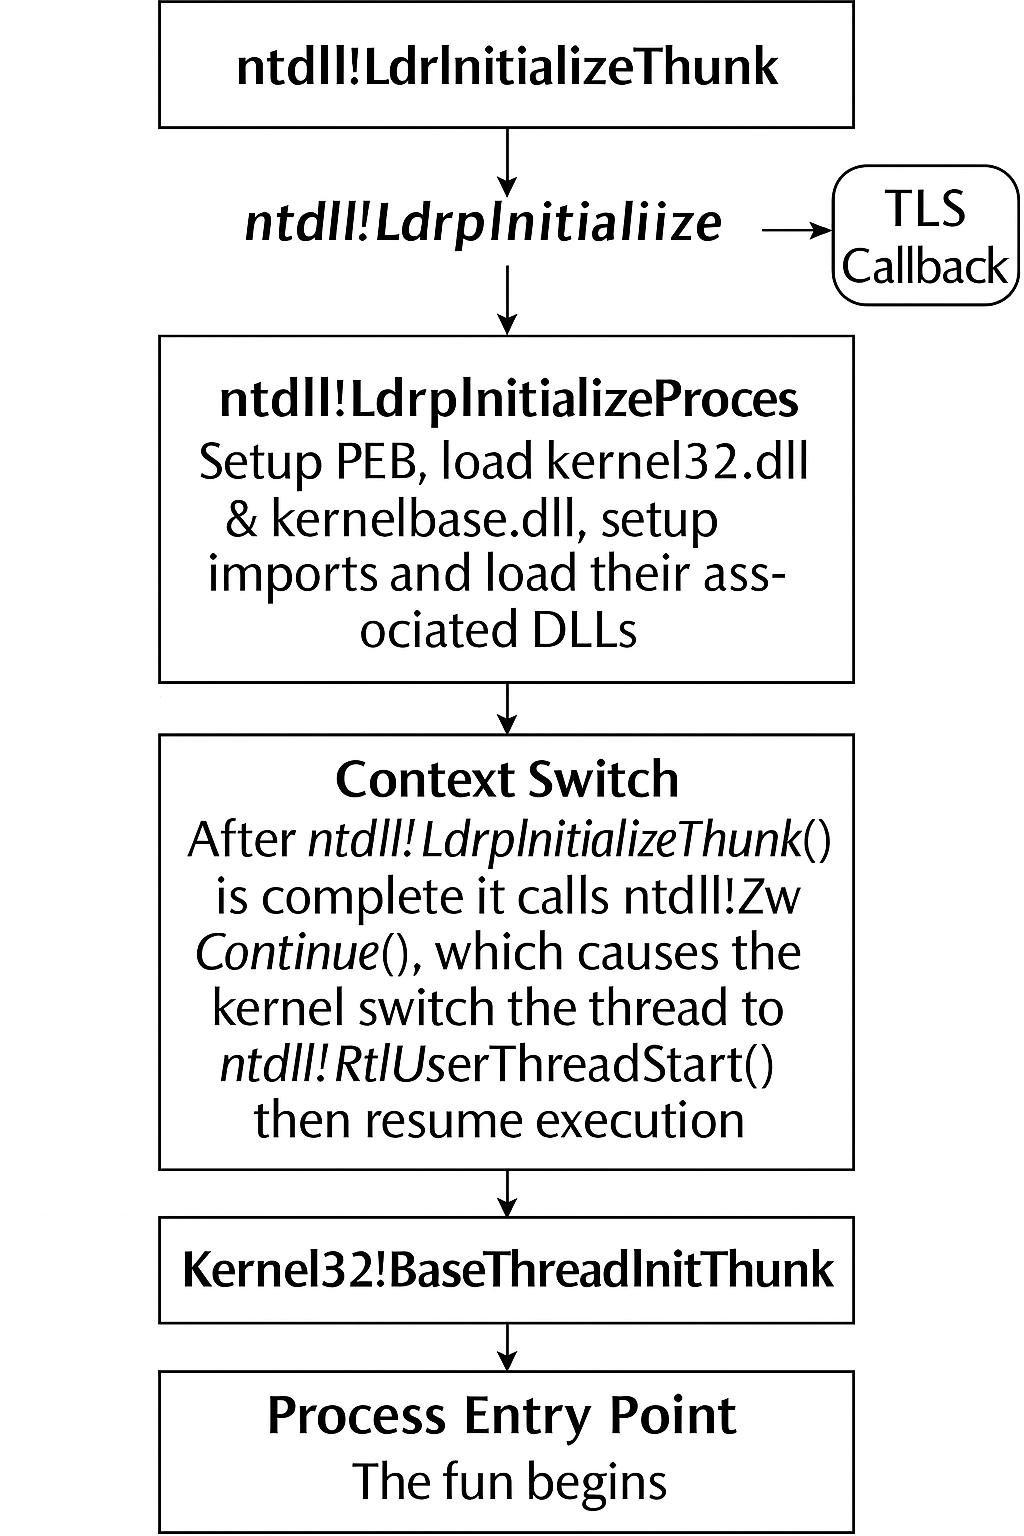
\includegraphics[width=0.45\textwidth]{images/tls_callback.png}
        \caption{Windows thread initialization with TLS Callback execution highlighted.}
        \label{fig:tls-callback-diagram}
\end{figure}
\end{comment}

If an injected DLL includes TLS callbacks and they are not properly removed or disabled, the cheat risks being detected immediately during process initialization.

\subsection*{Start Address Integrity Checks}

Beyond startup checks, anti-cheats like VAC continuously monitor thread creation during gameplay.  
A common detection method involves checking the \textbf{start address} of each thread.

\begin{tcolorbox}[colback=gray!10, colframe=gray!10, boxrule=0pt, sharp corners, width=\linewidth, left=1mm, right=1mm, top=0.5mm, bottom=0.5mm]
    \textbf{What is a Start Address?} \\
    The start address is the location in memory where a thread begins its execution. Legitimate threads typically start inside official game modules, such as \texttt{client.dll} or other trusted libraries.
\end{tcolorbox}    

If a thread is found starting at an address like \texttt{0x5F3A0000}, which falls outside any known game module (e.g., not within \texttt{client.dll}), it is highly suspicious and often indicates injected code or shellcode execution.

This method is particularly effective at catching poorly concealed code injections or shellcode execution.

\subsection*{VMT Hook Detection}

Another detection strategy focuses on the integrity of in-game objects.

In object-oriented engines, game entities typically use \textbf{Virtual Method Tables (VMTs)} to organize their functions.

\begin{tcolorbox}[colback=gray!10, colframe=gray!10, boxrule=0pt, sharp corners, width=\linewidth, left=1mm, right=1mm, top=0.5mm, bottom=0.5mm]
\textbf{What is a Virtual Method Table (VMT)?} \\
A VMT is a table used in object-oriented programming to map object methods to their actual function addresses. By modifying a VMT, an attacker can hijack how a game object behaves.
\end{tcolorbox}

Cheats often modify these tables to hijack behaviors, such as altering rendering or player input.

Anti-cheats like VAC can identify tampered VMTs by verifying:

\begin{itemize}
    \item Whether the VMT points to unexpected memory regions.
    \item Whether the methods referenced fall outside legitimate game or system modules.
\end{itemize}

\begin{figure}[h!]
    \centering
    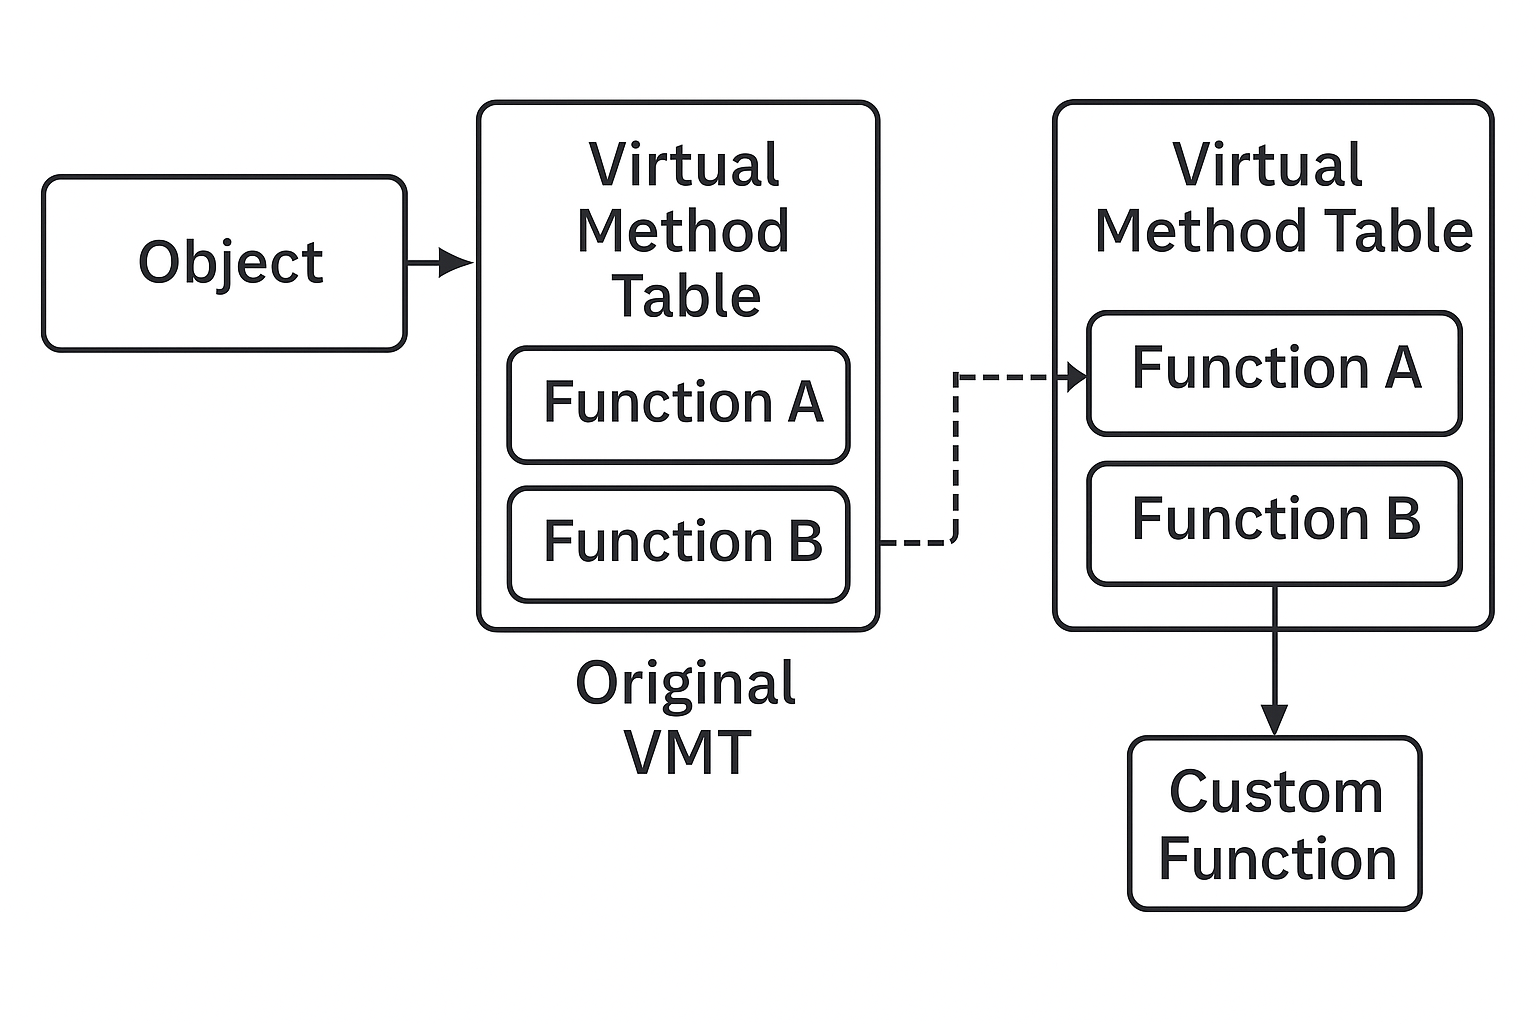
\includegraphics[width=0.65\textwidth]{images/vmthooking.png}
    \caption{Example of VMT Hooking.}
    \label{fig:vmt-hooking-diagram}
\end{figure}

Due to their clear memory footprint, traditional VMT hooks are now considered relatively high-risk in modern cheat development.

\section{Evasion Techniques Used by Cheats}

As anti-cheat systems like VAC become more sophisticated in their detection capabilities, cheat developers continuously adapt by designing increasingly advanced evasion techniques.  
These strategies aim to minimize the attack surface, avoid triggering heuristic scans, and maintain stealth even under active monitoring.

In this section, we present and explain some of the most common methods used to evade detection.


\subsection*{Suppressing TLS Callbacks}

To avoid early-stage detection, cheats often remove or disable the TLS callback directory from their injected DLLs.  
By doing so, they prevent anti-cheats from executing inspection routines before the cheat is fully concealed.

\subsection*{Thread Hijacking and Return Address Spoofing}

Instead of creating new threads—an action easily spotted—some cheats \textbf{hijack existing game threads}.

\begin{tcolorbox}[colback=gray!10, colframe=gray!10, boxrule=0pt, sharp corners, width=\linewidth, left=1mm, right=1mm, top=0.5mm, bottom=0.5mm]
\textbf{What is Thread Hijacking?} \\
Thread hijacking involves pausing an existing, legitimate thread, changing its instruction pointer to execute custom code, and then resuming it—making it harder for anti-cheats to notice any new activity.
\end{tcolorbox}

To further hide execution, cheats use \textbf{return address spoofing}—manipulating the call stack to make it appear that their code was naturally invoked from within the game’s legitimate modules.

\subsection*{Start Address Redirection via ROP Gadgets}

A more advanced and stealthy method used by cheats involves \textbf{Return-Oriented Programming (ROP)}.

\begin{tcolorbox}[colback=gray!10, colframe=gray!10, boxrule=0pt, sharp corners, width=\linewidth, left=1mm, right=1mm, top=0.5mm, bottom=0.5mm]
\textbf{What is a ROP Gadget?} \\
A ROP gadget is a small snippet of code already present in trusted modules, such as the game executable or Windows libraries. These snippets typically end with control transfer instructions like \texttt{ret} (return) or \texttt{jmp reg}.
\end{tcolorbox}

Instead of directly calling malicious code (which could be easily detected), cheats use ROP gadgets to build fake call chains.  
This way, their execution path appears legitimate, making detection much harder.

\paragraph{Stack Alignment and Shadow Space.}

In 64-bit Windows environments, the calling convention (\texttt{Microsoft x64}) imposes strict rules on how functions must be called, particularly regarding the stack layout:

\begin{itemize}
    \item \textbf{Stack Alignment}: Before calling any function, the stack pointer (\texttt{rsp}) must be 16-byte aligned. This ensures that SIMD instructions (like \texttt{movaps}) and internal ABI requirements function correctly.
    \item \textbf{Shadow Space}: Additionally, 32 bytes must be reserved on the stack for the called function to use freely. This space is used to store register parameters or local variables.
\end{itemize}

Failure to meet these requirements can cause functions to crash, corrupt data, or behave unpredictably.  
Moreover, violating calling conventions can raise suspicion in anti-cheat systems performing runtime integrity checks.

To correctly prepare the stack for a spoofed or redirected call during ROP, cheats must adjust the stack before jumping to the target function.

Here is an example of a minimal x64 call stub that correctly aligns the stack and reserves the required shadow space:

\begin{lstlisting}[style=asmstyle]
sub rsp, 0x28               ; reserve 32 bytes shadow space + align stack (16-byte alignment)
mov rax, 0xFFAAFFAAFFAAFFAA ; address of the ROP gadget to act as a fake return address
push rax                    ; push the fake return address onto the stack
mov rax, 0xFFAAFFAAFFAAFFAA ; address of the actual target function to execute
jmp rax                     ; jump to the real function
\end{lstlisting}

This setup ensures that:

\begin{itemize}
    \item The stack is properly aligned (after \texttt{sub rsp, 0x28}).
    \item A valid-looking return address (pointing to a trusted ROP gadget) is pushed.
    \item The function call structure looks legitimate, reducing the risk of detection.
\end{itemize}

Thus, when the called function finishes and executes a \texttt{ret} instruction, it returns to a safe, believable address instead of crashing or exposing the cheat.

\paragraph{Detection Vectors.}

While ROP techniques are highly stealthy, anti-cheats can still perform \textbf{stack walking}—analyzing the call stack at runtime to detect inconsistencies, fake return addresses, or suspicious memory regions.

\paragraph{Practical Implementations.}

Open-source projects like \texttt{x86RetSpoof} by danielkrupinski offer practical examples of return address spoofing.  
However, professional cheats often use customized ROP implementations tailored to specific games like CS2 for maximum stealth.

\section{Extended VAC Capabilities and Developer Countermeasures}

Beyond basic memory and thread inspections, \textbf{Valve Anti-Cheat (VAC)} extends its detection efforts through broader system monitoring.  
It actively scans the file system looking for known cheat artifacts, inspects running processes for suspicious memory regions or injected modules, monitors the Windows registry for abnormal entries, and tracks inter-process activity to detect unauthorized access to the game.

This expanded approach allows VAC to move beyond simple memory analysis, building a more complete picture of system behavior and making traditional static cheats easier to detect.

In response, cheat developers have introduced a range of countermeasures aimed at staying hidden.  
String encryption is commonly used to obfuscate identifiable patterns in memory. Name randomization changes module and window identifiers dynamically to avoid blacklists.  
More advanced techniques include polymorphic code, which mutates the cheat at runtime to evade pattern detection, and fileless execution, where the cheat operates entirely from memory without touching the disk.  
Memory cleansing after injection further minimizes visible traces that could expose the cheat during active scanning.

Ultimately, the ongoing battle between anti-cheat technologies and cheat developers drives constant innovation on both sides.  
As VAC strengthens its methods to detect unauthorized activity, cheats evolve to become more stealthy, adaptive, and resilient — ensuring that the arms race in competitive gaming security remains in constant motion.
